\documentclass[11pt]{article}

\usepackage[margin=1in]{geometry}
\usepackage{setspace}
\onehalfspacing
\usepackage{graphicx}
\usepackage{listings}
\usepackage{float}

% DOCUMENT INFORMATION =================================================
\title {ECEN 423: Introduction to Digital Systems Design \\ North Carolina Agricultural and Technical State University \\ Department of Electrical and Computer Engineering} % Declare Title
\author{Chris Cannon} % Declare authors
\date{February 8, 2018}
% ======================================================================

\begin{document}
	
\maketitle

\begin{center}
	Homework 3
\end{center}

%================Examples====================
%\begin{figure}[H]
%\begin{center}
%	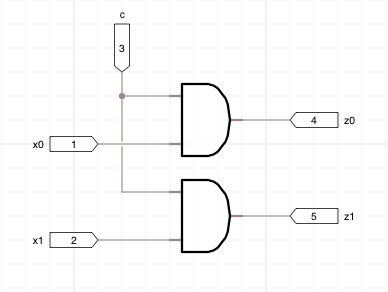
\includegraphics{img3_1.png}
%	\caption{\label{fig:triStateSchematic} Schematic for 2-bit Tri-State buffer assuming active HIGH.}
%\end{center}
%\end{figure}
%==========================================

\section{Problem 6.7 Multiples of Three}
Design and test a logical circuit that will output HIGH when a 4-bit input represents a multiple of 3. Inputs that should trigger HIGH are listed in Table ~\ref{tab:multThree}.

\begin{table}
\begin{center}
	\begin{tabular}{| l |}
		\hline
		0011 \\ \hline
		0110 \\ \hline
		1001 \\ \hline
		1100 \\ \hline
		1111 \\ \hline
	\end{tabular}
	\caption{\label{tab:multThree}4-bit multiples of three.}
\end{center}	
\end{table}

\subsection{VHDL Code for Multiples of Three}

\begin{lstlisting}[language=VHDL]
entity multiple_three is
	port(a : in bit_vector(3 downto 0); x : out bit);
end multiple_three;

architecture mult_arch of multiple_three is
	begin
		x <= '1' when (a = "0011" or a = "0110" or a = "1001" or a = "1100" or a = "1111") else '0';
end mult_arch;
\end{lstlisting}

\end{document}